% Options for packages loaded elsewhere
\PassOptionsToPackage{unicode}{hyperref}
\PassOptionsToPackage{hyphens}{url}
%
\documentclass[
  ignorenonframetext,
]{beamer}
\usepackage{pgfpages}
\setbeamertemplate{caption}[numbered]
\setbeamertemplate{caption label separator}{: }
\setbeamercolor{caption name}{fg=normal text.fg}
\beamertemplatenavigationsymbolsempty
% Prevent slide breaks in the middle of a paragraph
\widowpenalties 1 10000
\raggedbottom
\setbeamertemplate{part page}{
  \centering
  \begin{beamercolorbox}[sep=16pt,center]{part title}
    \usebeamerfont{part title}\insertpart\par
  \end{beamercolorbox}
}
\setbeamertemplate{section page}{
  \centering
  \begin{beamercolorbox}[sep=12pt,center]{part title}
    \usebeamerfont{section title}\insertsection\par
  \end{beamercolorbox}
}
\setbeamertemplate{subsection page}{
  \centering
  \begin{beamercolorbox}[sep=8pt,center]{part title}
    \usebeamerfont{subsection title}\insertsubsection\par
  \end{beamercolorbox}
}
\AtBeginPart{
  \frame{\partpage}
}
\AtBeginSection{
  \ifbibliography
  \else
    \frame{\sectionpage}
  \fi
}
\AtBeginSubsection{
  \frame{\subsectionpage}
}
\usepackage{amsmath,amssymb}
\usepackage{iftex}
\ifPDFTeX
  \usepackage[T1]{fontenc}
  \usepackage[utf8]{inputenc}
  \usepackage{textcomp} % provide euro and other symbols
\else % if luatex or xetex
  \usepackage{unicode-math} % this also loads fontspec
  \defaultfontfeatures{Scale=MatchLowercase}
  \defaultfontfeatures[\rmfamily]{Ligatures=TeX,Scale=1}
\fi
\usepackage{lmodern}
\usetheme[]{Boadilla}
\ifPDFTeX\else
  % xetex/luatex font selection
\fi
% Use upquote if available, for straight quotes in verbatim environments
\IfFileExists{upquote.sty}{\usepackage{upquote}}{}
\IfFileExists{microtype.sty}{% use microtype if available
  \usepackage[]{microtype}
  \UseMicrotypeSet[protrusion]{basicmath} % disable protrusion for tt fonts
}{}
\makeatletter
\@ifundefined{KOMAClassName}{% if non-KOMA class
  \IfFileExists{parskip.sty}{%
    \usepackage{parskip}
  }{% else
    \setlength{\parindent}{0pt}
    \setlength{\parskip}{6pt plus 2pt minus 1pt}}
}{% if KOMA class
  \KOMAoptions{parskip=half}}
\makeatother
\usepackage{xcolor}
\newif\ifbibliography
\usepackage{color}
\usepackage{fancyvrb}
\newcommand{\VerbBar}{|}
\newcommand{\VERB}{\Verb[commandchars=\\\{\}]}
\DefineVerbatimEnvironment{Highlighting}{Verbatim}{commandchars=\\\{\}}
% Add ',fontsize=\small' for more characters per line
\usepackage{framed}
\definecolor{shadecolor}{RGB}{248,248,248}
\newenvironment{Shaded}{\begin{snugshade}}{\end{snugshade}}
\newcommand{\AlertTok}[1]{\textcolor[rgb]{0.94,0.16,0.16}{#1}}
\newcommand{\AnnotationTok}[1]{\textcolor[rgb]{0.56,0.35,0.01}{\textbf{\textit{#1}}}}
\newcommand{\AttributeTok}[1]{\textcolor[rgb]{0.13,0.29,0.53}{#1}}
\newcommand{\BaseNTok}[1]{\textcolor[rgb]{0.00,0.00,0.81}{#1}}
\newcommand{\BuiltInTok}[1]{#1}
\newcommand{\CharTok}[1]{\textcolor[rgb]{0.31,0.60,0.02}{#1}}
\newcommand{\CommentTok}[1]{\textcolor[rgb]{0.56,0.35,0.01}{\textit{#1}}}
\newcommand{\CommentVarTok}[1]{\textcolor[rgb]{0.56,0.35,0.01}{\textbf{\textit{#1}}}}
\newcommand{\ConstantTok}[1]{\textcolor[rgb]{0.56,0.35,0.01}{#1}}
\newcommand{\ControlFlowTok}[1]{\textcolor[rgb]{0.13,0.29,0.53}{\textbf{#1}}}
\newcommand{\DataTypeTok}[1]{\textcolor[rgb]{0.13,0.29,0.53}{#1}}
\newcommand{\DecValTok}[1]{\textcolor[rgb]{0.00,0.00,0.81}{#1}}
\newcommand{\DocumentationTok}[1]{\textcolor[rgb]{0.56,0.35,0.01}{\textbf{\textit{#1}}}}
\newcommand{\ErrorTok}[1]{\textcolor[rgb]{0.64,0.00,0.00}{\textbf{#1}}}
\newcommand{\ExtensionTok}[1]{#1}
\newcommand{\FloatTok}[1]{\textcolor[rgb]{0.00,0.00,0.81}{#1}}
\newcommand{\FunctionTok}[1]{\textcolor[rgb]{0.13,0.29,0.53}{\textbf{#1}}}
\newcommand{\ImportTok}[1]{#1}
\newcommand{\InformationTok}[1]{\textcolor[rgb]{0.56,0.35,0.01}{\textbf{\textit{#1}}}}
\newcommand{\KeywordTok}[1]{\textcolor[rgb]{0.13,0.29,0.53}{\textbf{#1}}}
\newcommand{\NormalTok}[1]{#1}
\newcommand{\OperatorTok}[1]{\textcolor[rgb]{0.81,0.36,0.00}{\textbf{#1}}}
\newcommand{\OtherTok}[1]{\textcolor[rgb]{0.56,0.35,0.01}{#1}}
\newcommand{\PreprocessorTok}[1]{\textcolor[rgb]{0.56,0.35,0.01}{\textit{#1}}}
\newcommand{\RegionMarkerTok}[1]{#1}
\newcommand{\SpecialCharTok}[1]{\textcolor[rgb]{0.81,0.36,0.00}{\textbf{#1}}}
\newcommand{\SpecialStringTok}[1]{\textcolor[rgb]{0.31,0.60,0.02}{#1}}
\newcommand{\StringTok}[1]{\textcolor[rgb]{0.31,0.60,0.02}{#1}}
\newcommand{\VariableTok}[1]{\textcolor[rgb]{0.00,0.00,0.00}{#1}}
\newcommand{\VerbatimStringTok}[1]{\textcolor[rgb]{0.31,0.60,0.02}{#1}}
\newcommand{\WarningTok}[1]{\textcolor[rgb]{0.56,0.35,0.01}{\textbf{\textit{#1}}}}
\usepackage{longtable,booktabs,array}
\usepackage{calc} % for calculating minipage widths
\usepackage{caption}
% Make caption package work with longtable
\makeatletter
\def\fnum@table{\tablename~\thetable}
\makeatother
\usepackage{graphicx}
\makeatletter
\def\maxwidth{\ifdim\Gin@nat@width>\linewidth\linewidth\else\Gin@nat@width\fi}
\def\maxheight{\ifdim\Gin@nat@height>\textheight\textheight\else\Gin@nat@height\fi}
\makeatother
% Scale images if necessary, so that they will not overflow the page
% margins by default, and it is still possible to overwrite the defaults
% using explicit options in \includegraphics[width, height, ...]{}
\setkeys{Gin}{width=\maxwidth,height=\maxheight,keepaspectratio}
% Set default figure placement to htbp
\makeatletter
\def\fps@figure{htbp}
\makeatother
\usepackage{soul}
\setlength{\emergencystretch}{3em} % prevent overfull lines
\providecommand{\tightlist}{%
  \setlength{\itemsep}{0pt}\setlength{\parskip}{0pt}}
\setcounter{secnumdepth}{-\maxdimen} % remove section numbering
\setbeamertemplate{itemize item}[circle]
\setbeamertemplate{enumerate item}[circle]
\usepackage{tikz}
\usetikzlibrary{arrows.meta,calc,tikzmark,fit}
\newcommand{\Rlogo}{\includegraphics[height=1em]{/Library/Frameworks/R.framework/Resources/doc/html/logo.jpg}}
\newcommand{\R}{\texttt{R}}
\newcommand{\highlight}[1]{\StringTok{#1}}
\newcommand{\important}[1]{\AlertTok{#1}}
\newcommand{\fade}[1]{\textcolor[rgb]{0.66,0.66,0.66}{#1}}
\newcommand{\annote}[1]{{\footnotesize #1}}
\newcommand{\name}[1]{\textit{texttt{\VariableTok{#1}}}}
\ifLuaTeX
  \usepackage{selnolig}  % disable illegal ligatures
\fi
\IfFileExists{bookmark.sty}{\usepackage{bookmark}}{\usepackage{hyperref}}
\IfFileExists{xurl.sty}{\usepackage{xurl}}{} % add URL line breaks if available
\urlstyle{same}
\hypersetup{
  pdftitle={A Gentle Introduction to R},
  pdfauthor={Jonathan Whiteley},
  hidelinks,
  pdfcreator={LaTeX via pandoc}}

\title{A Gentle Introduction to R}
\author{Jonathan Whiteley}
\date{2023-08-09}

\begin{document}
\frame{\titlepage}

\begin{frame}{Pop Quiz}
\protect\hypertarget{pop-quiz}{}
{\footnotesize \textcolor[rgb]{0.66,0.66,0.66}{We will review these \textit{at the end}, so you can see how much you have learned.}}

\begin{itemize}
\tightlist
\item
  What does `CRAN' stand for?
\item
  Why is it named `\(\texttt{R}\)'?
\item
  How can you use \(\texttt{R}\) \emph{interactively}?
\item
  How do you find out what a function does \& how to use it?
\item
  How do you store values to re-use later?
\item
  True or False: Warnings can be ignored, but an Error means I made a
  mistake.
\item
  True or False: Error messages will tell me how to fix the problem.
\end{itemize}

~

\begin{block}{Answer in the chat:}
\protect\hypertarget{answer-in-the-chat}{}
What emoji best describes your current mood or state of mind?
\end{block}
\end{frame}

\begin{frame}[fragile]{Introductions}
\protect\hypertarget{introductions}{}
\begin{itemize}
\tightlist
\item
  Name
\item
  Pronouns
\item
  Job Title, role
\item
  Have you used \(\texttt{R}\) before?
\item
  Have you used a programming language before?
\item
  \emph{optional}: a hobby or activity you enjoy?
\end{itemize}

\note{Other icebreaker questions:

\begin{itemize}
\tightlist
\item
  Favourite candy or treat as a child?
\item
  Favourite music band or genre?
\item
  Favourite book?
\item
  Highlight of the past month / year (personal or professional)?
\end{itemize}

If available on platform, online polls:

\begin{itemize}
\tightlist
\item
  Where are you joining from?
\item
  Have you used \texttt{R} before?
\item
  Have you used a programming language before?
\end{itemize}

If a chat is available, put answer to a question there:

\begin{itemize}
\tightlist
\item
  What emoji best describes your current mood or state of mind?
\item
  Favourite emoji?
\end{itemize}

More icebreaker ideas:

\begin{itemize}
\tightlist
\item
  \url{https://blog.slido.com/virtual-icebreakers/}
\item
  \url{https://www.mural.co/blog/virtual-meeting-ice-breakers}
\end{itemize}}
\end{frame}

\begin{frame}{ Icebreaker activity}
\protect\hypertarget{icebreaker-activity}{}
\begin{columns}[T]
\begin{column}{0.5\textwidth}
\textbf{What is this?}\\
1--3 word description, for~example:

\begin{itemize}
\tightlist
\item
  ``This is grey''
\item
  ``This looks uncomfortable''
\end{itemize}

\hfill\break
On your turn:

\begin{enumerate}
\item
  Previous person's name
\item
  Their answer to the question
\item
  Your name
\item
  Your answer
\item
  Name of the person to go next
\end{enumerate}
\end{column}

\begin{column}{0.5\textwidth}
\begin{figure}
\centering
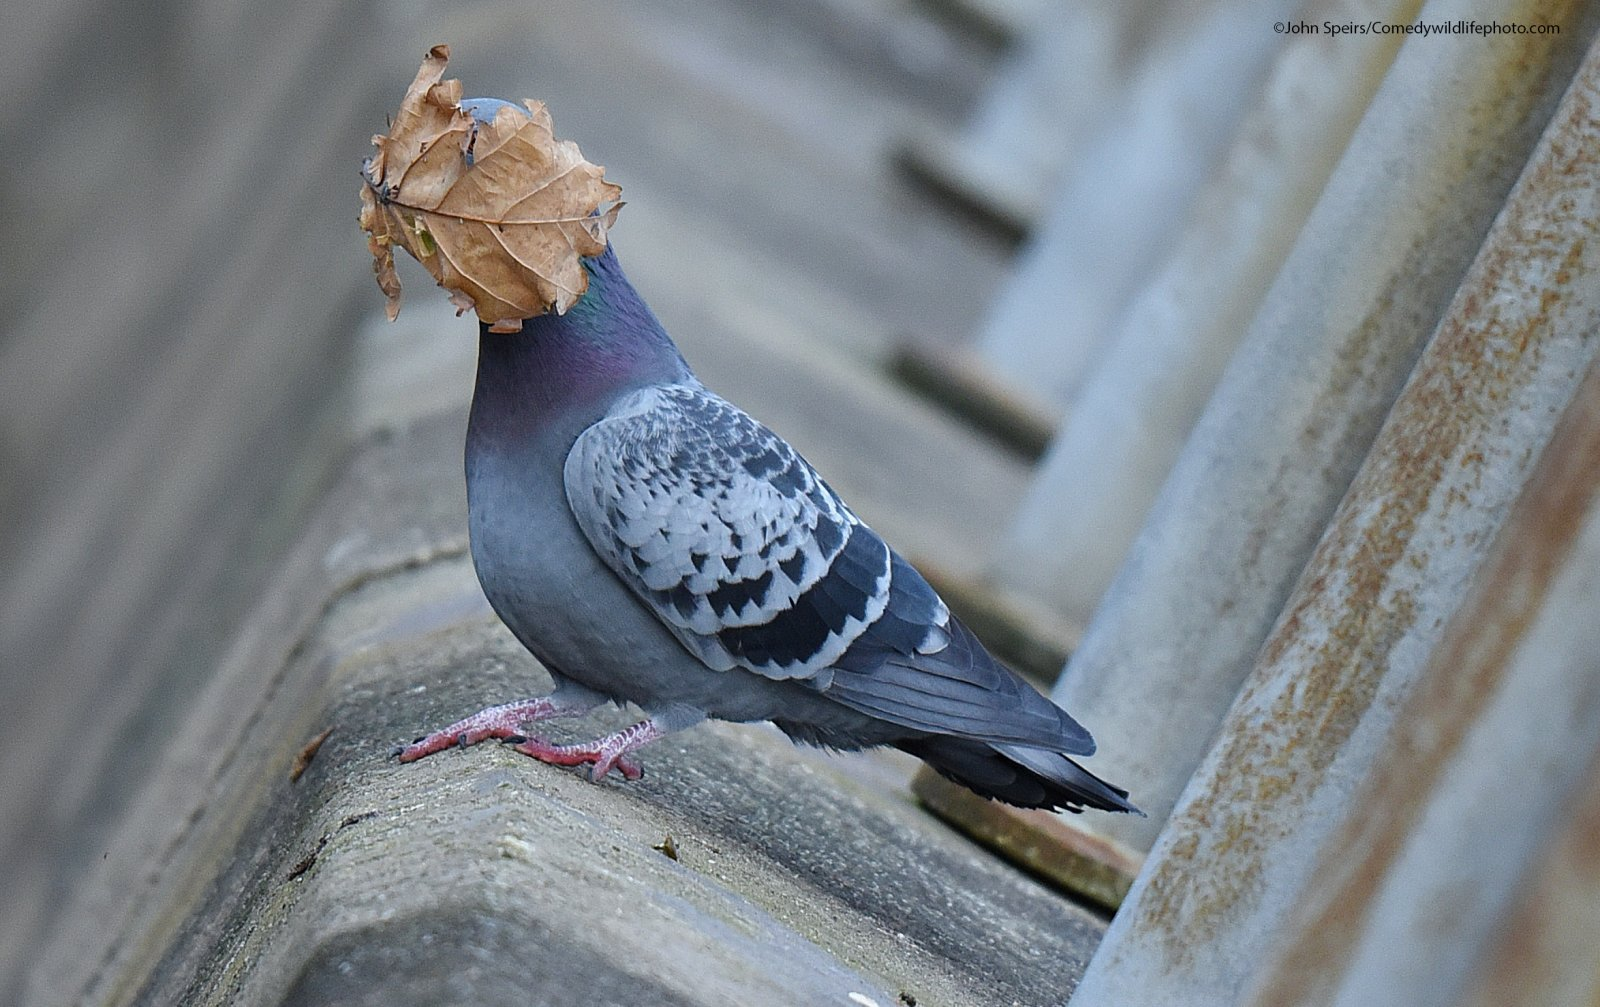
\includegraphics[width=1\textwidth,height=\textheight]{images/john-speirs_i-guess-summers-over.jpg}
\caption{What is this?\\
©
\href{https://www.comedywildlifephoto.com/gallery/comedy-wildlife-2021-competition-winners.php}{John
Speirs/Comedywildlifephoto.com}}
\end{figure}
\end{column}
\end{columns}
\end{frame}

\begin{frame}{Learning Objectives}
\protect\hypertarget{learning-objectives}{}
\begin{itemize}
\tightlist
\item
  Get familiar with the
  \includegraphics[width=\textwidth,height=1em]{/Library/Frameworks/R.framework/Resources/doc/html/logo.jpg}\footnote<.->{The
    R logo
    (\(\includegraphics[height=1em]{/Library/Frameworks/R.framework/Resources/doc/html/logo.jpg}\))
    is \href{https://www.r-project.org/logo/}{© 2016 The R Foundation}
    and used as-is under the terms of the
    \href{https://creativecommons.org/licenses/by-sa/4.0/}{\textbf{CC-BY-SA
    4.0} license}} \emph{interface}
\item
  Use technical \emph{terms} for \(\texttt{R}\) concepts
\item
  Enter \emph{commands}

  \begin{itemize}
  \tightlist
  \item
    use \(\texttt{R}\) interactively: understand input \& output
  \item
    use some common \emph{functions}
  \end{itemize}
\item
  Get familiar with `\(\texttt{R}\) objects'

  \begin{itemize}
  \tightlist
  \item
    store \& retrieve values
  \end{itemize}
\item
  Understand \emph{Errors}, \emph{Warnings}, and \emph{Messages}
\item
  How to get Help
\end{itemize}
\end{frame}

\begin{frame}[fragile]{Why is it named `\(\texttt{R}\)'?}
\protect\hypertarget{why-is-it-named-textttr}{}
\begin{enumerate}
\item
  \textbf{\(\texttt{R}\)} started as an \emph{open-source}
  implementation of the\\
  \textbf{\texttt{S}} statistical computing language
  (S-PLUS)\footnote<.->{\url{https://www.r-project.org/about.html}}

  \begin{itemize}
  \item
    \texttt{S} was created at Bell Laboratories in 1976\footnote<.->{\url{https://en.wikipedia.org/wiki/S_(programming_language)}}
  \item
    \(\texttt{R}\) was based on the \texttt{S} syntax (mostly v3), but
    works very differently ``under the hood''.
  \end{itemize}
\item
  \textbf{\(\texttt{R}\)} was created by \ul{\textbf{R}}oss Ihaka and
  \ul{\textbf{R}}obert Gentleman --- aka ``R \& R''\footnote<.->{\url{https://www.r-project.org/contributors.html}}
  --- at the University of Aukland in the early 1990s.
\end{enumerate}

\hfill\break
\emph{Read more about the history of \(\texttt{R}\) on
\href{https://en.wikipedia.org/wiki/R_(programming_language)\#History}{Wikipedia}}\footnote<.->{\url{https://en.wikipedia.org/wiki/R_(programming_language)\#History}}
\end{frame}

\begin{frame}{The
\(\includegraphics[height=1em]{/Library/Frameworks/R.framework/Resources/doc/html/logo.jpg}\)
Interface}
\protect\hypertarget{the-includegraphicsheight1emlibraryframeworksr.frameworkresourcesdochtmllogo.jpg-interface}{}
\begin{itemize}
\tightlist
\item
  `base \(\texttt{R}\)' has a slightly different interface for each
  \textbf{O}perating \textbf{S}ystem (OS)

  \begin{itemize}
  \tightlist
  \item
    GUI = \textbf{G}raphical \textbf{U}ser \textbf{I}nterface
  \end{itemize}
\item
  \(\texttt{R}\) can also run inside of a terminal (no GUI) or other
  software (different GUI).
\end{itemize}

\begin{block}{\href{https://en.wikipedia.org/wiki/Integrated_development_environment}{\textbf{I}ntegrated
\textbf{D}evelopment \textbf{E}nvironment} (IDE)}
\protect\hypertarget{integrated-development-environment-ide}{}
\begin{itemize}
\tightlist
\item
  An IDE is like an extra interface layer on top of `base
  \(\texttt{R}\)'
\item
  IDEs often add convenient tools to make writing code easier (e.g.,
  syntax highlighting), and for developing larger projects with multiple
  files.
\item
  \textbf{\href{https://posit.co/products/open-source/rstudio/}{RStudio}}
  is one of the most popular cross-platform IDEs for \(\texttt{R}\).

  \begin{itemize}
  \tightlist
  \item
    RStudio is available in open source (free/libre) and
    commercial\footnote<.->{for organizations not able to use software
      licensed with AGPL} editions.
  \end{itemize}
\end{itemize}
\end{block}
\end{frame}

\begin{frame}{A quick tour of the `base \(\texttt{R}\) GUI'}
\protect\hypertarget{a-quick-tour-of-the-base-textttr-gui}{}
\begin{figure}
\centering
\begin{tikzpicture}[overlay/.style={ultra thick, rounded corners, draw=red, fill=white, fill opacity=0.5, text opacity=1},
                    note/.style={align=center, font=\Large\bfseries}]
  \node[anchor=south west,inner sep=0] (image) at (0,0) {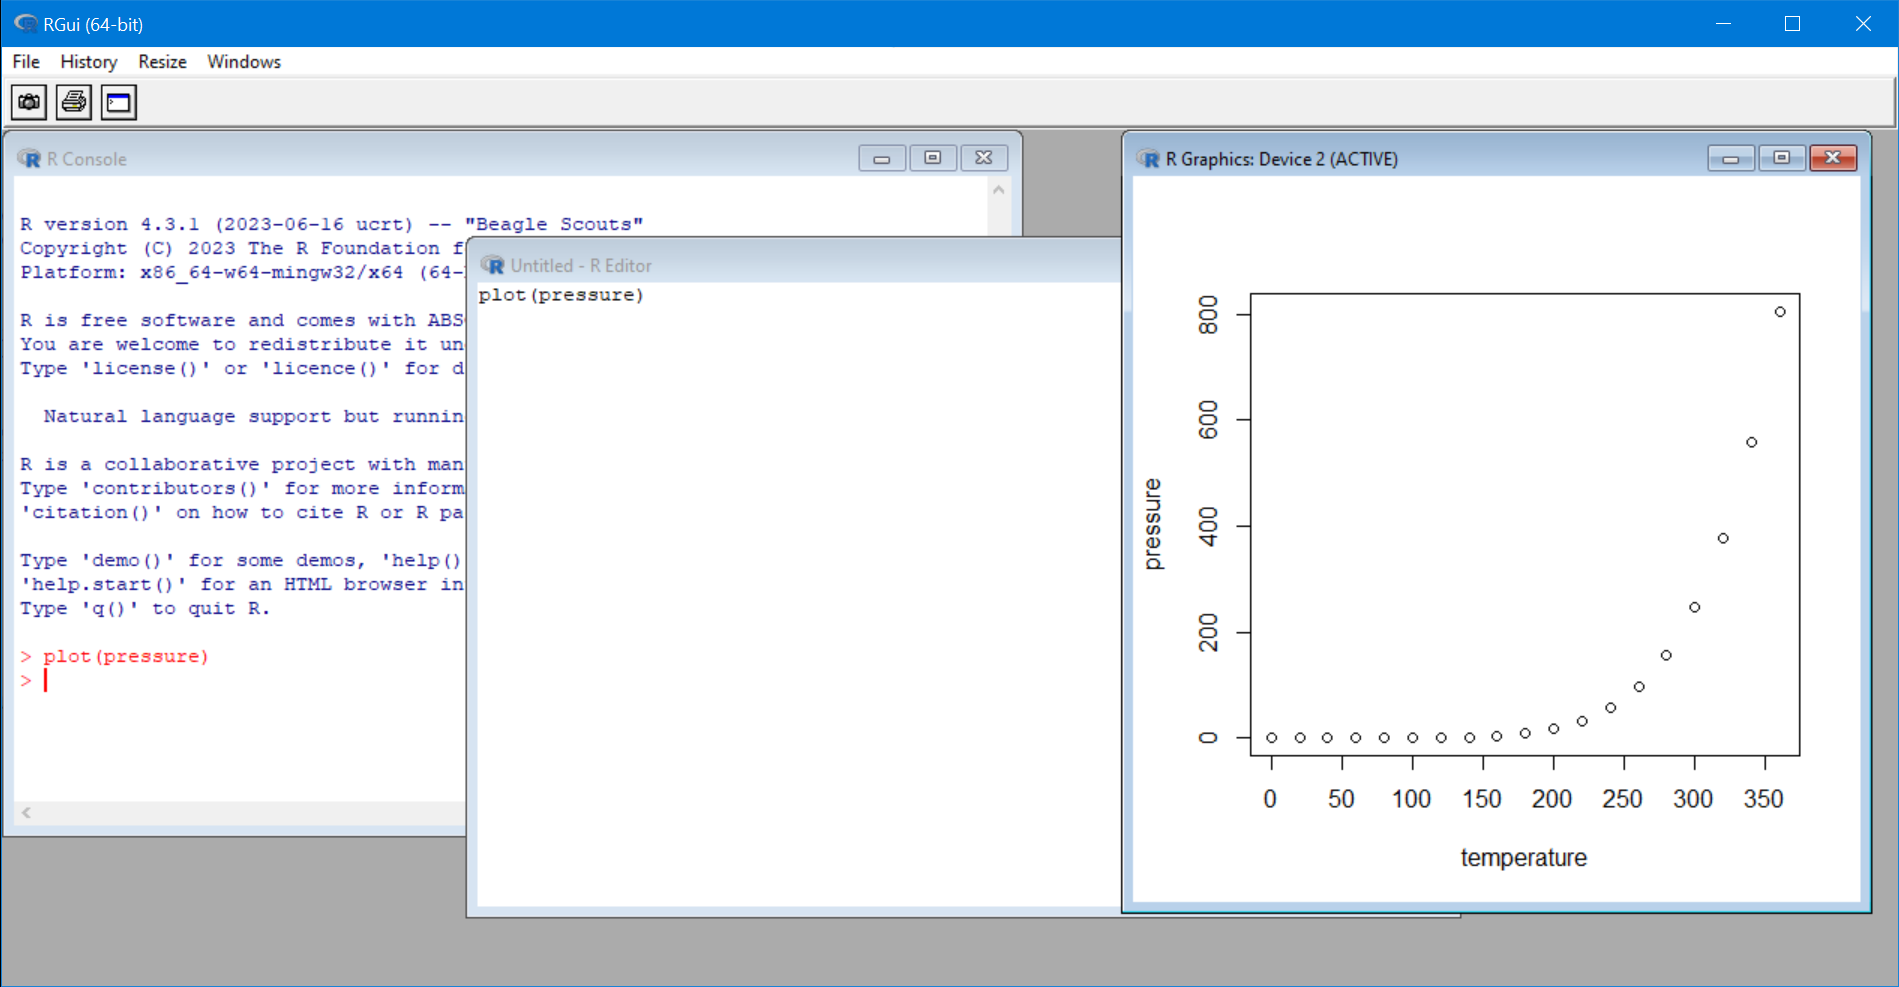
\includegraphics[width=0.9\textwidth]{images/R-screenshot-script-plot-win.png}};
  \begin{scope}[x={(image.south east)},y={(image.north west)}]
    \draw[overlay] (0,0.15) rectangle (0.54,0.87);
    \node[note] at (0.14,0.27) {console};
    \draw[overlay] (0.245,0.065) rectangle (0.585,0.76);
    \node[note] at (0.415,0.41) {source};
    \draw[overlay] (0.588,0.07) rectangle (0.987,0.87);
    \node[note] at (0.788,0.47) {plot\\ window};
  \end{scope}
\end{tikzpicture}
\caption{Screenshot of the R GUI in Windows.}
\end{figure}
\end{frame}

\begin{frame}{A quick tour of RStudio}
\protect\hypertarget{a-quick-tour-of-rstudio}{}
\begin{columns}[T]
\begin{column}{0.75\textwidth}
The RStudio GUI has 4 `panes' that contain `tabs'.

\begin{figure}
\centering
\begin{tikzpicture}[overlay/.style={ultra thick, draw=red, fill=white, fill opacity=0.5, text opacity=1},
                    circler/.style={radius=3ex},
                    note/.style={align=center, font=\Large\bfseries}]
  \node[anchor=south west,inner sep=0] (image) at (0,0) {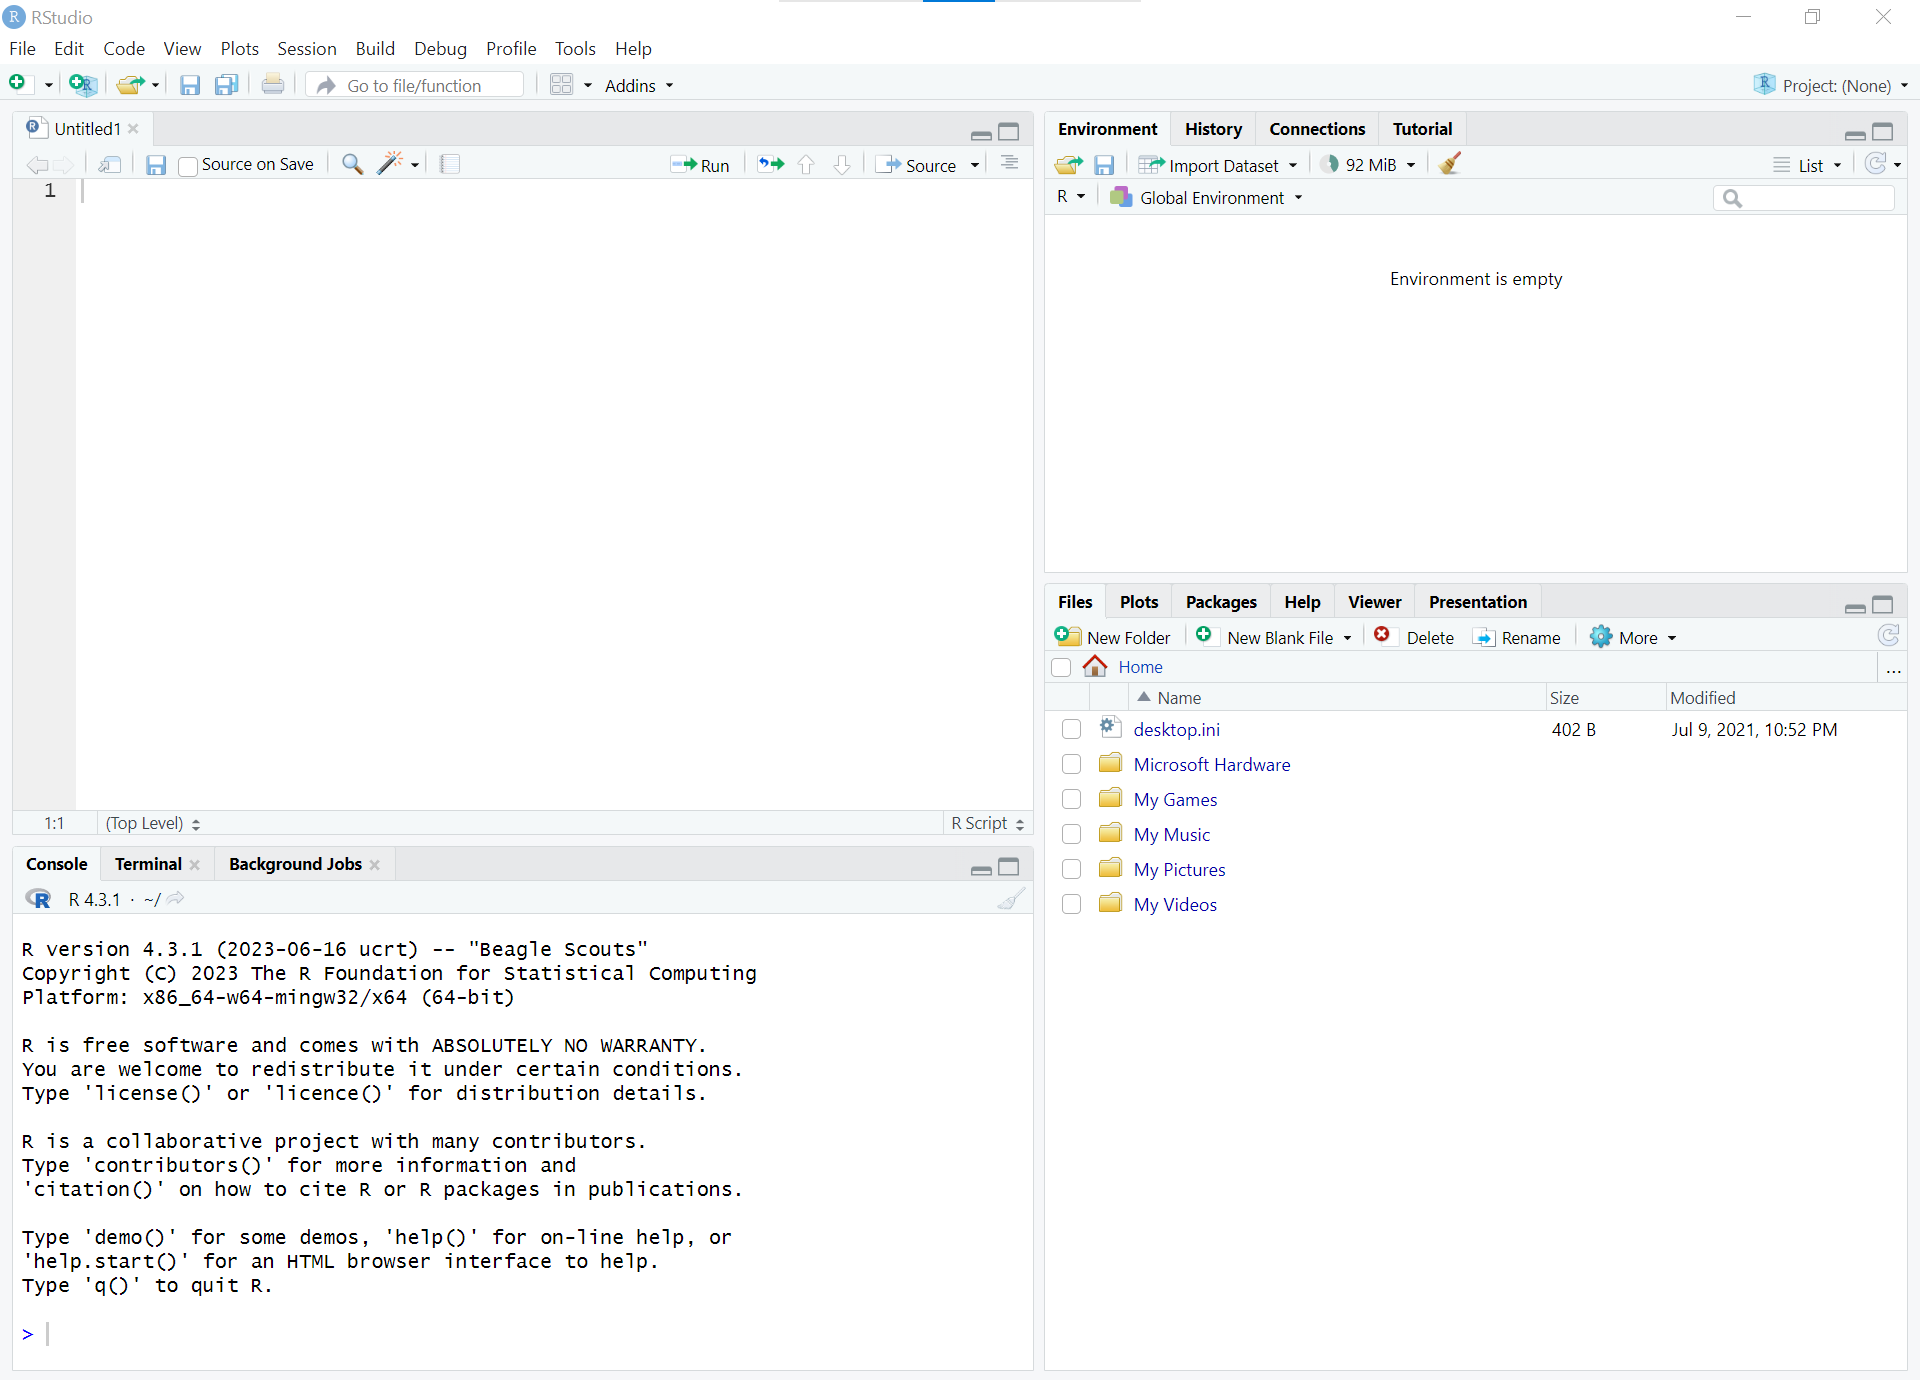
\includegraphics[width=\textwidth]{images/RStudio-screenshot-4pane-default.png}};
  \begin{scope}[x={(image.south east)},y={(image.north west)}]
    \draw[overlay] (0.45,0.7) circle[circler] node[note] {1};
    \draw[overlay] (0.45,0.2) circle[radius=3ex] node[note] {2};
    \draw[overlay] (0.80,0.7) circle[radius=3ex] node[note] {3};
    \draw[overlay] (0.80,0.2) circle[radius=3ex] node[note] {4};
  \end{scope}
\end{tikzpicture}
\caption{Screenshot of RStudio (default layout).}
\end{figure}
\end{column}

\begin{column}{0.25\textwidth}
left:

\begin{enumerate}
\item
  top: \textbf{Source}\footnote<.->{empty until you create or open a
    file}
\item
  bottom: \textbf{Console, Terminal, \ldots{}}
\end{enumerate}

right:

\begin{enumerate}
\setcounter{enumi}{2}
\item
  top:\\
  \textbf{Environment, History, \ldots{}}
\item
  bottom: \textbf{Files, Plots, Help, \ldots{}}
\end{enumerate}
\end{column}
\end{columns}
\end{frame}

\begin{frame}{Interacting with
\(\includegraphics[height=1em]{/Library/Frameworks/R.framework/Resources/doc/html/logo.jpg}\)}
\protect\hypertarget{interacting-with-includegraphicsheight1emlibraryframeworksr.frameworkresourcesdochtmllogo.jpg}{}
\begin{itemize}
\item
  Regardless of the GUI, you interact with \(\texttt{R}\) primarily
  using a \emph{command~line}

  \begin{itemize}
  \tightlist
  \item
    aka a \ul{c}ommand \ul{l}ine \ul{i}nterface (cli)
  \item
    the command line is usually in the \emph{console}
  \end{itemize}
\item
  ``Question-and-Answer Model''

  \begin{itemize}
  \item
    You ask \(\texttt{R}\) to do something (a \emph{command}),\\
    \hspace*{0.333em}\hspace*{0.333em}\hspace*{0.333em}\hspace*{0.333em}\hspace*{0.333em}and
    \(\texttt{R}\) tells you the answer (\emph{result}).
  \end{itemize}
\item
  Instructions are given to \(\texttt{R}\) using the \emph{R language}.
\end{itemize}

\note{R is designed so that users can start by using it
\emph{interactively} (what we will do today), and then gradually use it
for more programming as their needs and skills grow.

\begin{itemize}
\tightlist
\item
  Not ``point-and-click'': no menus or wizards to guide you through
  steps of an analysis or procedure.
\end{itemize}}
\end{frame}

\begin{frame}{The
\(\includegraphics[height=1em]{/Library/Frameworks/R.framework/Resources/doc/html/logo.jpg}\)
console}
\protect\hypertarget{the-includegraphicsheight1emlibraryframeworksr.frameworkresourcesdochtmllogo.jpg-console}{}
The \emph{console} is a window or pane where you will find:

\begin{itemize}
\item
  The \emph{command line}

  \begin{itemize}
  \tightlist
  \item
    where you will enter commands for \(\texttt{R}\) to run
  \end{itemize}
\item
  Results of commands and other output
\item
  Messages, Warnings, and Errors
\end{itemize}
\end{frame}

\begin{frame}[fragile]{The
\(\includegraphics[height=1em]{/Library/Frameworks/R.framework/Resources/doc/html/logo.jpg}\)
command-line}
\protect\hypertarget{the-includegraphicsheight1emlibraryframeworksr.frameworkresourcesdochtmllogo.jpg-command-line}{}
\begin{itemize}
\item
  The command \emph{prompt} normally looks like this:

\begin{Shaded}
\begin{Highlighting}[]
\NormalTok{\textgreater{}}
\end{Highlighting}
\end{Shaded}

  {\footnotesize (the colour varies depending on the interface)}

  \begin{itemize}
  \tightlist
  \item
    This is \(\texttt{R}\)'s way of saying ``I am ready to accept new
    commands''.
  \item
    Type a new command on the line after this prompt (i.e.,
    \emph{input}).
  \end{itemize}
\item
  \textbf{Press \AlertTok{\texttt{return}}/\AlertTok{\texttt{enter}} to
  \emph{run} the current \emph{command} }
\item
  If you can still edit the command next to the prompt, then it has not
  been submitted to \(\texttt{R}\) to execute (it is still waiting for
  input).
\item
  If the last prompt is not empty (i.e., there is text beside it)\\
  \emph{and} you cannot edit what is beside the prompt,\\
  it means \(\texttt{R}\) is still running the last command and is not
  ready to accept a new command yet.

  \begin{itemize}
  \tightlist
  \item
    Wait for a new empty prompt to appear before entering the next
    command.
  \end{itemize}
\end{itemize}
\end{frame}

\begin{frame}[fragile]{The
\(\includegraphics[height=1em]{/Library/Frameworks/R.framework/Resources/doc/html/logo.jpg}\)
command-line (continued)}
\protect\hypertarget{the-includegraphicsheight1emlibraryframeworksr.frameworkresourcesdochtmllogo.jpg-command-line-continued}{}
\begin{itemize}
\item
  If the prompt looks like this:

\begin{Shaded}
\begin{Highlighting}[]
\NormalTok{+}
\end{Highlighting}
\end{Shaded}

  it means the last command was \emph{incomplete} and \(\texttt{R}\) is
  waiting for more input.\\
  \(\texttt{R}\) will not do anything until the command is completed or
  cancelled.

  \begin{itemize}
  \tightlist
  \item
    This usually means you forgot a closing\\
    \emph{quote} \AlertTok{\texttt{"}}, \emph{parenthesis}
    \AlertTok{\texttt{(}}, \emph{bracket} \AlertTok{\texttt{[}}, or
    \emph{brace} \AlertTok{\texttt{\{}}
  \end{itemize}
\item
  \StringTok{You can \textit{cancel} the current command at any time by pressing \texttt{escape}}
  (\AlertTok{\texttt{esc}})
\end{itemize}
\end{frame}

\begin{frame}[fragile]{Input \& Output}
\protect\hypertarget{input-output}{}
In this presentation,

\begin{itemize}
\item
  \emph{commands} that can be entered in the \emph{command-line} look
  like this:

\hypertarget{format_input}{%
\label{format_input}}%
\begin{Shaded}
\begin{Highlighting}[]
\NormalTok{Input (commands)}
\end{Highlighting}
\end{Shaded}

  \begin{itemize}
  \tightlist
  \item
    You can try these yourself!
  \end{itemize}
\item
  Expected output (results) look like this:

\begin{verbatim}
## Output (results)
\end{verbatim}
\end{itemize}
\end{frame}

\begin{frame}{\(\includegraphics[height=1em]{/Library/Frameworks/R.framework/Resources/doc/html/logo.jpg}\)
offers suggestions}
\protect\hypertarget{includegraphicsheight1emlibraryframeworksr.frameworkresourcesdochtmllogo.jpg-offers-suggestions}{}
Read the opening message carefully.

\begin{figure}
\centering
\begin{tikzpicture}[overlay/.style={ultra thick, rounded corners, draw=red, fill=none},
                    note/.style={anchor=west, align=left, font=\Large\bfseries},
                    ->/.style={ultra thick, red, -{Latex}[round]}]
  \node[anchor=south west,inner sep=0] (image) at (0,0) {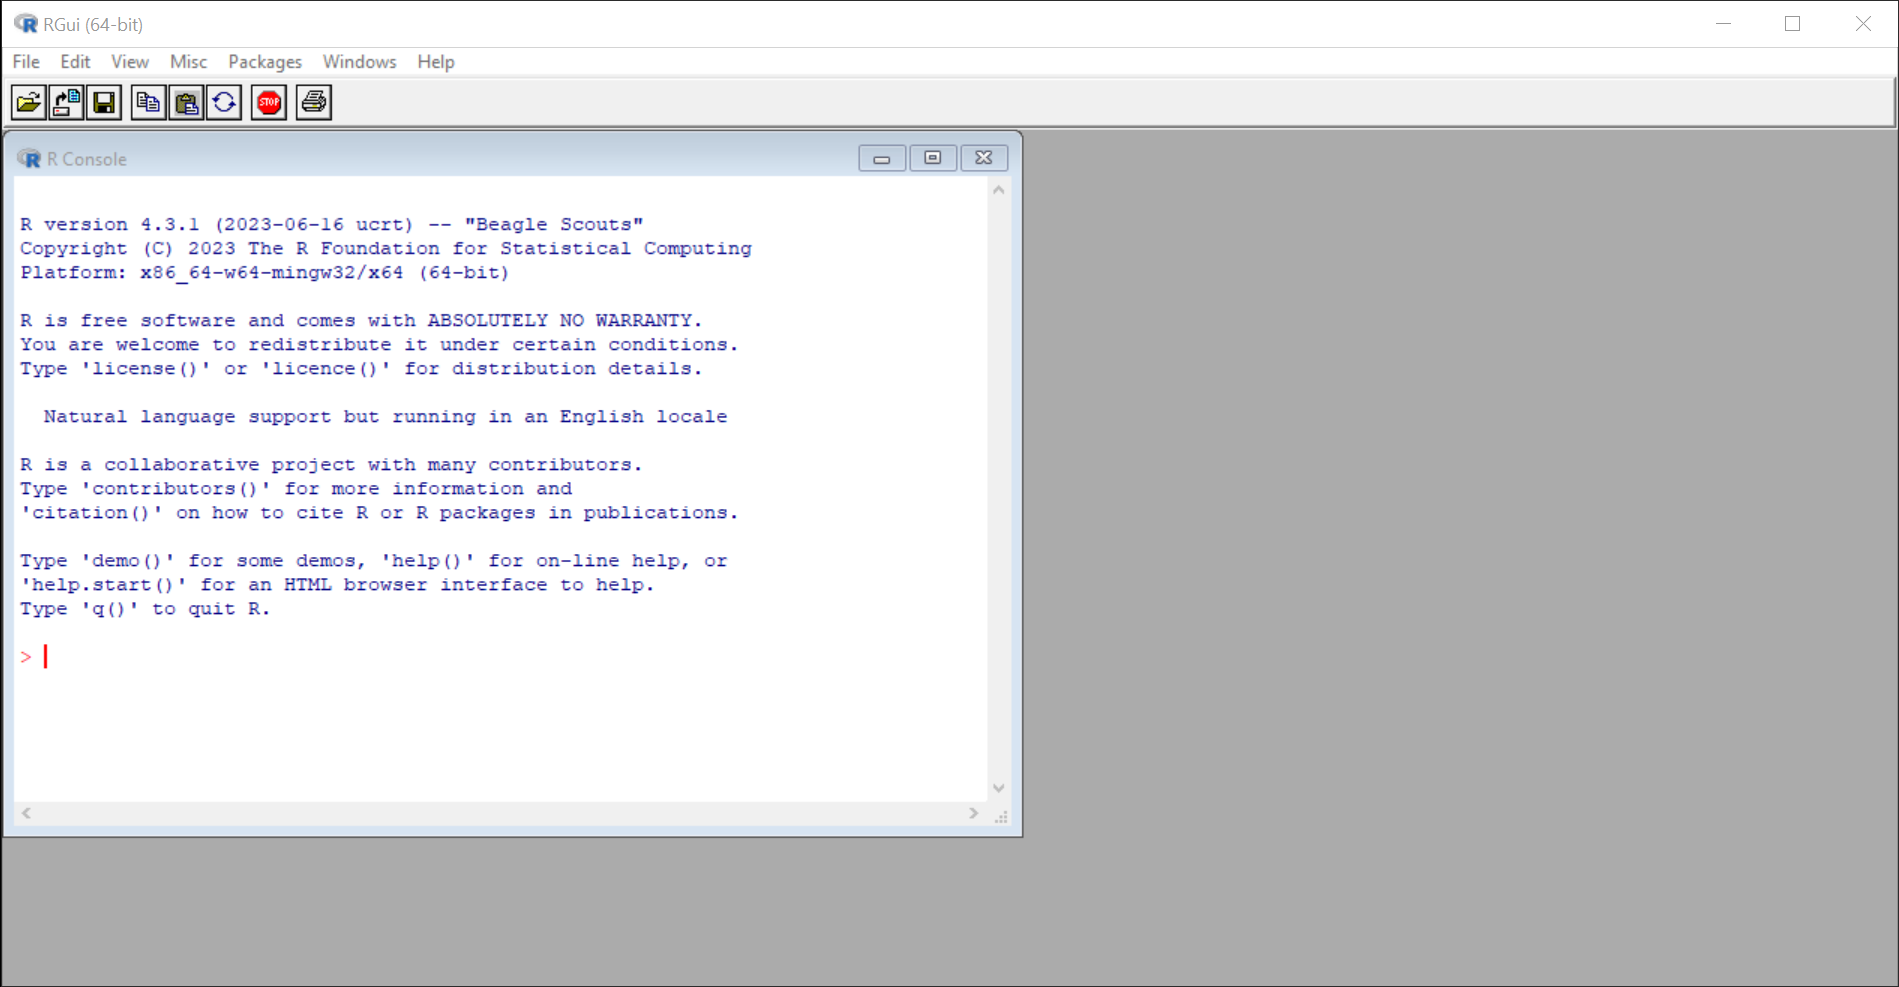
\includegraphics[width=0.9\textwidth]{images/R-screenshot-win-default}};
  \begin{scope}[x={(image.south east)},y={(image.north west)}]
    \node (rect) [overlay, fit={(0,0.36) (0.42,0.46)}, inner sep=0] {};
    \node (note)  [note, text width=12em] at (0.55,0.41) {\textcolor[rgb]{0.60,0.00,0.00}{$\R$ offers suggestions to start with}};
    \draw [->] (note.west) -> (rect.east);
  \end{scope}
\end{tikzpicture}
\caption{$\texttt{R}$ offers suggestions of commands to \KeywordTok{\texttt{Type}} in the console when it starts.}
\end{figure}
\end{frame}

\begin{frame}[fragile]{\(\includegraphics[height=1em]{/Library/Frameworks/R.framework/Resources/doc/html/logo.jpg}\)
is a show-off}
\protect\hypertarget{includegraphicsheight1emlibraryframeworksr.frameworkresourcesdochtmllogo.jpg-is-a-show-off}{}
\begin{longtable}[]{@{}
  >{\raggedright\arraybackslash}p{(\columnwidth - 2\tabcolsep) * \real{0.2625}}
  >{\raggedright\arraybackslash}p{(\columnwidth - 2\tabcolsep) * \real{0.7375}}@{}}
\toprule\noalign{}
\endhead
\begin{minipage}[t]{\linewidth}\raggedright
\begin{Shaded}
\begin{Highlighting}[]
\FunctionTok{demo}\NormalTok{(graphics)}
\end{Highlighting}
\end{Shaded}
\end{minipage} & \begin{minipage}[t]{\linewidth}\raggedright
\begin{itemize}
\tightlist
\item
  some plots and graphs that can be made with \(\texttt{R}\)
\end{itemize}
\end{minipage} \\
\begin{minipage}[t]{\linewidth}\raggedright
\begin{Shaded}
\begin{Highlighting}[]
\FunctionTok{demo}\NormalTok{(image)}
\end{Highlighting}
\end{Shaded}
\end{minipage} & \begin{minipage}[t]{\linewidth}\raggedright
\begin{itemize}
\tightlist
\item
  image-like graphics and maps that can be produced with \(\texttt{R}\)
\end{itemize}
\end{minipage} \\
\begin{minipage}[t]{\linewidth}\raggedright
\begin{Shaded}
\begin{Highlighting}[]
\FunctionTok{demo}\NormalTok{(lm.glm)}
\end{Highlighting}
\end{Shaded}
\end{minipage} & \begin{minipage}[t]{\linewidth}\raggedright
\begin{itemize}
\tightlist
\item
  a demonstration of linear modelling \& GLMs
\end{itemize}
\end{minipage} \\
\begin{minipage}[t]{\linewidth}\raggedright
\begin{Shaded}
\begin{Highlighting}[]
\FunctionTok{demo}\NormalTok{()}
\end{Highlighting}
\end{Shaded}
\end{minipage} & \begin{minipage}[t]{\linewidth}\raggedright
\begin{itemize}
\tightlist
\item
  a list of available demos
\end{itemize}
\end{minipage} \\
\begin{minipage}[t]{\linewidth}\raggedright
\begin{Shaded}
\begin{Highlighting}[]
\FunctionTok{help.start}\NormalTok{()}
\end{Highlighting}
\end{Shaded}
\end{minipage} & \begin{minipage}[t]{\linewidth}\raggedright
\hfill\break
\textbf{←} A great place to start,\\
\hspace*{0.333em}\hspace*{0.333em}\hspace*{0.333em}\hspace*{0.333em}especially
if you are comfortable reading\\
\hspace*{0.333em}\hspace*{0.333em}\hspace*{0.333em}\hspace*{0.333em}documentation
for a programming language.\\
\hspace*{0.333em}\hspace*{0.333em}\hspace*{0.333em}\hspace*{0.333em}More
on this later.
\end{minipage} \\
\bottomrule\noalign{}
\end{longtable}

\begin{block}{Note}
\protect\hypertarget{note}{}
\texttt{R}{} will not only show the output, but also \emph{the code used
to produce it}.
\end{block}
\end{frame}

\begin{frame}[fragile]{\(\includegraphics[height=1em]{/Library/Frameworks/R.framework/Resources/doc/html/logo.jpg}\)
is a show-off (alt)}
\protect\hypertarget{includegraphicsheight1emlibraryframeworksr.frameworkresourcesdochtmllogo.jpg-is-a-show-off-alt}{}
\begin{columns}[T]
\begin{column}{0.4\textwidth}
\begin{Shaded}
\begin{Highlighting}[]
\FunctionTok{demo}\NormalTok{(graphics)  }
\FunctionTok{demo}\NormalTok{(image)     }
\FunctionTok{demo}\NormalTok{(lm.glm)    }
\FunctionTok{demo}\NormalTok{()          }

\FunctionTok{help.start}\NormalTok{()    }
\end{Highlighting}
\end{Shaded}

\hfill\break
\tikzmarknode{n1}{A} great place to start, especially if you are
comfortable reading documentation for a programming language.\\
More on this later.
\end{column}

\begin{column}{0.6\textwidth}
\begin{itemize}

\item[\tikzmarknode{b1}{$\bullet$}]
  some plots and graphs that can be made with $\texttt{R}$

\item[\tikzmarknode{b2}{$\bullet$}]
  image-like graphics and maps that can be made with $\texttt{R}$

\item[\tikzmarknode{b3}{$\bullet$}]
  a demonstration of linear modelling \& GLMs

\item[\tikzmarknode{b4}{$\bullet$}]
  a list of available demos

\end{itemize}

\hfill\break

\begin{block}{Note}
\protect\hypertarget{note-1}{}
\texttt{R}{} will not only show the output, but also\\
\emph{the code used to produce it}.
\end{block}
\end{column}
\end{columns}

\begin{tikzpicture}[remember picture, overlay]
  \draw [ultra thick, gray, -{Latex}] ( $ (n1.north) +(0,2pt) $ ) -- ++(0,4ex);
  \draw [ultra thick, gray, -{Latex}] (b1.west) -- ++(-14ex,-1.5ex);
  \draw [ultra thick, gray, -{Latex}] (b2.west) -- ++(-17ex,1.5ex);
  \draw [ultra thick, gray, -{Latex}] (b3.west) -- ++(-16ex,4ex);
  \draw [ultra thick, gray, -{Latex}] (b4.west) -- ++(-23ex,7ex);
\end{tikzpicture}
\end{frame}

\begin{frame}[fragile]{\(\includegraphics[height=1em]{/Library/Frameworks/R.framework/Resources/doc/html/logo.jpg}\)
is a calculator}
\protect\hypertarget{includegraphicsheight1emlibraryframeworksr.frameworkresourcesdochtmllogo.jpg-is-a-calculator}{}
\begin{columns}[T]
\begin{column}{0.5\textwidth}
\begin{Shaded}
\begin{Highlighting}[]
\DecValTok{1} \SpecialCharTok{+} \DecValTok{1}
\end{Highlighting}
\end{Shaded}

\begin{verbatim}
## [1] 2
\end{verbatim}

\begin{Shaded}
\begin{Highlighting}[]
\DecValTok{2} \SpecialCharTok{*} \DecValTok{2}
\end{Highlighting}
\end{Shaded}

\begin{verbatim}
## [1] 4
\end{verbatim}

\begin{Shaded}
\begin{Highlighting}[]
\DecValTok{2} \SpecialCharTok{\^{}} \DecValTok{3}
\end{Highlighting}
\end{Shaded}

\begin{verbatim}
## [1] 8
\end{verbatim}
\end{column}

\begin{column}{0.5\textwidth}
\begin{Shaded}
\begin{Highlighting}[]
\DecValTok{10} \SpecialCharTok{{-}} \DecValTok{1}
\end{Highlighting}
\end{Shaded}

\begin{verbatim}
## [1] 9
\end{verbatim}

\begin{Shaded}
\begin{Highlighting}[]
\DecValTok{8} \SpecialCharTok{/} \DecValTok{2}
\end{Highlighting}
\end{Shaded}

\begin{verbatim}
## [1] 4
\end{verbatim}

\begin{Shaded}
\begin{Highlighting}[]
\FunctionTok{sqrt}\NormalTok{(}\DecValTok{9}\NormalTok{)}
\end{Highlighting}
\end{Shaded}

\begin{verbatim}
## [1] 3
\end{verbatim}
\end{column}
\end{columns}

\begin{itemize}
\tightlist
\item
  These are \emph{expressions}
\item
  \emph{Expressions} are \emph{evaluated}, and the \emph{value} (result)
  is \emph{returned}\\
  (sometimes \emph{invisibly})
\end{itemize}

\note{The bullet points are accurate, but I note that the
\href{https://cran.r-project.org/doc/manuals/r-release/R-lang.html}{R
Language Definition} distinguishes between `expressions', which are
actually a type of object, and `statements' (see s2.1.3 `Language
objects', s2.1.4 `Expression objects'):

\begin{itemize}
\tightlist
\item
  An \emph{expression} \[object?\] contains one or more statements.
\item
  A statement is a syntactically correct collection of tokens.
\item
  Expression objects are special language objects which contain parsed
  but unevaluated R statements.
\item
  ``an expression object can contain several such expressions'' (not
  clear)
\end{itemize}

Therefore, my understanding is that a \emph{statement} is parsed (by the
R parser), which results in an unevaluated \emph{expression} (an object
of mode ``expression''), which can in turn be evaluated (by `the
evaluator', such as \texttt{eval()}) to return the \emph{value}.

``All expressions have a value.'' (s3 `Evaluation of expressions')}
\end{frame}

\begin{frame}{\(\includegraphics[height=1em]{/Library/Frameworks/R.framework/Resources/doc/html/logo.jpg}\)
command-line tips}
\protect\hypertarget{includegraphicsheight1emlibraryframeworksr.frameworkresourcesdochtmllogo.jpg-command-line-tips}{}
\begin{itemize}
\item
  With the cursor next to the empty prompt (\OtherTok{\texttt{>}}),\\
  use the up \& down \AlertTok{arrow keys} (↑↓) to re-produce previous
  commands.
\item
  This lets you ``scroll through your \emph{command history}''.
\item
  Press \AlertTok{up} (\AlertTok{$\uparrow$}) once, and you get the last
  command you entered\\
  without having to copy \& paste.
\end{itemize}
\end{frame}

\begin{frame}[fragile]{Symbolic \emph{variables}}
\protect\hypertarget{symbolic-variables}{}
\begin{itemize}
\tightlist
\item
  You can store values (\emph{objects}) in symbolic variables
  (\emph{names}) using an \emph{assignment operator}:
\end{itemize}

\begin{longtable}[]{@{}ll@{}}
\toprule\noalign{}
\endhead
\VERB|\OtherTok{\textless{}{-}}| & assign the \emph{value} on the
\textbf{right} to the \emph{name} on the \textbf{left} \\
\bottomrule\noalign{}
\end{longtable}

\begin{columns}[T]
\begin{column}{0.5\textwidth}
\begin{itemize}
\tightlist
\item
  Names can include:
\end{itemize}

\begin{longtable}[]{@{}ll@{}}
\toprule\noalign{}
\endhead
letters & \StringTok{\texttt{a-z A-Z}} \\
numbers & \StringTok{\texttt{0-9}} \\
periods & \StringTok{\texttt{.}} \\
underscores & \StringTok{\texttt{\_}} \\
\bottomrule\noalign{}
\end{longtable}

\begin{itemize}
\tightlist
\item
  Names \emph{should begin with a \textbf{\StringTok{letter}}}.
\end{itemize}
\end{column}

\begin{column}{0.5\textwidth}
\begin{Shaded}
\begin{Highlighting}[]
\NormalTok{A }\OtherTok{\textless{}{-}} \DecValTok{10}
\NormalTok{B }\OtherTok{\textless{}{-}} \DecValTok{10} \SpecialCharTok{*} \DecValTok{10}
\NormalTok{A\_log }\OtherTok{\textless{}{-}} \FunctionTok{log}\NormalTok{(A)}
\NormalTok{B.seq }\OtherTok{\textless{}{-}} \DecValTok{1}\SpecialCharTok{:}\NormalTok{B}

\FunctionTok{assign}\NormalTok{(}\StringTok{\textquotesingle{}x\textquotesingle{}}\NormalTok{, }\DecValTok{3}\NormalTok{)}
\end{Highlighting}
\end{Shaded}
\end{column}
\end{columns}
\end{frame}

\begin{frame}[fragile]{Retrieve values}
\protect\hypertarget{retrieve-values}{}
When a variable \emph{name} is evaluated, it returns the stored
\emph{value}.

\begin{columns}[T]
\begin{column}{0.5\textwidth}
\begin{Shaded}
\begin{Highlighting}[]
\NormalTok{A}
\end{Highlighting}
\end{Shaded}

\begin{verbatim}
## [1] 10
\end{verbatim}

\begin{Shaded}
\begin{Highlighting}[]
\NormalTok{A\_log}
\end{Highlighting}
\end{Shaded}

\begin{verbatim}
## [1] 2.303
\end{verbatim}
\end{column}

\begin{column}{0.5\textwidth}
\begin{Shaded}
\begin{Highlighting}[]
\NormalTok{B}
\end{Highlighting}
\end{Shaded}

\begin{verbatim}
## [1] 100
\end{verbatim}

\begin{Shaded}
\begin{Highlighting}[]
\NormalTok{x}
\end{Highlighting}
\end{Shaded}

\begin{verbatim}
## [1] 3
\end{verbatim}
\end{column}
\end{columns}

\begin{Shaded}
\begin{Highlighting}[]
\NormalTok{B.seq}
\end{Highlighting}
\end{Shaded}

\begin{verbatim}
##   [1]   1   2   3   4   5   6   7   8   9  10  11  12
##  [13]  13  14  15  16  17  18  19  20  21  22  23  24
##  [25]  25  26  27  28  29  30  31  32  33  34  35  36
##  [37]  37  38  39  40  41  42  43  44  45  46  47  48
##  [49]  49  50  51  52  53  54  55  56  57  58  59  60
##  [61]  61  62  63  64  65  66  67  68  69  70  71  72
##  [73]  73  74  75  76  77  78  79  80  81  82  83  84
##  [85]  85  86  87  88  89  90  91  92  93  94  95  96
##  [97]  97  98  99 100
\end{verbatim}
\end{frame}

\begin{frame}[fragile]{Built-in variables}
\protect\hypertarget{built-in-variables}{}
Some words and letters already have values in \(\texttt{R}\)\\
and should \textbf{never be used as variable names}.

\begin{columns}[T]
\begin{column}{0.5\textwidth}
\begin{Shaded}
\begin{Highlighting}[]
\NormalTok{pi}
\end{Highlighting}
\end{Shaded}

\begin{verbatim}
## [1] 3.142
\end{verbatim}
\end{column}

\begin{column}{0.5\textwidth}
\begin{Shaded}
\begin{Highlighting}[]
\NormalTok{version}
\end{Highlighting}
\end{Shaded}

\begin{verbatim}
## ... information about 
## this version of R ...
\end{verbatim}
\end{column}
\end{columns}

\begin{Shaded}
\begin{Highlighting}[]
\NormalTok{letters}
\end{Highlighting}
\end{Shaded}

\begin{verbatim}
##  [1] "a" "b" "c" "d" "e" "f" "g" "h" "i" "j" "k" "l" "m"
## [14] "n" "o" "p" "q" "r" "s" "t" "u" "v" "w" "x" "y" "z"
\end{verbatim}

\begin{Shaded}
\begin{Highlighting}[]
\NormalTok{LETTERS}
\end{Highlighting}
\end{Shaded}

\begin{verbatim}
##  [1] "A" "B" "C" "D" "E" "F" "G" "H" "I" "J" "K" "L" "M"
## [14] "N" "O" "P" "Q" "R" "S" "T" "U" "V" "W" "X" "Y" "Z"
\end{verbatim}
\end{frame}

\begin{frame}{Reserved words}
\protect\hypertarget{reserved-words}{}
Some words and letters already have special meaning in the R language
(\emph{keywords}) and should \textbf{never be used as variable names}.
\end{frame}

\begin{frame}[fragile]{\protect\hyperlink{pop-quiz}{Quiz} Review}
\protect\hypertarget{quiz-review}{}
\note{\texttt{\#\#\ Answers\ (for\ discussion)}

answer in notes}
\end{frame}

\begin{frame}[fragile]{References \& More Information}
\protect\hypertarget{references-more-information}{}
\begin{Shaded}
\begin{Highlighting}[]
\FunctionTok{help.start}\NormalTok{()}
\end{Highlighting}
\end{Shaded}

Accessible from the screen above (offline):

\begin{itemize}
\tightlist
\item
  \href{https://cran.r-project.org/doc/manuals/r-release/R-intro.html}{An
  Introduction to R}
\item
  \href{https://cran.r-project.org/doc/manuals/r-release/R-lang.html}{The
  R Language Definition}
\end{itemize}

Online:

\begin{itemize}
\tightlist
\item
  \href{https://education.rstudio.com/}{RStudio Education}
  (\href{https://education.rstudio.com/}{education.rstudio.com})

  \begin{itemize}
  \tightlist
  \item
    tutorials, workshop materials, and other resources.
  \end{itemize}
\item
  \(\includegraphics[height=1em]{/Library/Frameworks/R.framework/Resources/doc/html/logo.jpg}\)
  \href{https://cran.r-project.org/manuals.html}{Manuals}
  (\url{https://cran.r-project.org/manuals.html})
\item
  \(\includegraphics[height=1em]{/Library/Frameworks/R.framework/Resources/doc/html/logo.jpg}\)
  \href{https://cran.r-project.org/other-docs.html}{Contributed
  Documentation}

  \begin{itemize}
  \tightlist
  \item
    e.g., \url{http://cran.r-project.org/doc/contrib/usingR.pdf}
  \end{itemize}
\item
  Internet search

  \begin{itemize}
  \tightlist
  \item
    \href{https://stackoverflow.com/questions/tagged/r}{Stack Overflow}
    (\href{https://stackoverflow.com/}{stackoverflow.com})
  \item
    \href{http://www.cookbook-r.com/}{Cookbook for R}
    (\href{http://www.cookbook-r.com/}{www.cookbook-r.com})
  \end{itemize}
\end{itemize}

\note{Other training materials and tutorials used as inspiration:

\begin{itemize}
\tightlist
\item
  \href{https://link.springer.com/book/10.1007/978-0-387-93837-0}{A
  Beginner's Guide to R}
\item
  \href{https://link.springer.com/book/10.1007/978-0-387-79054-1}{Introductory
  Statistics with R}
\item
  \href{https://education.rstudio.com/}{RStudio Education}
\item
  \url{https://rladiessydney.org/courses/ryouwithme/01-basicbasics-0/}
\item
  \url{https://moderndive.netlify.app/1-getting-started.html}
\item
  \url{https://cengel.github.io/R-intro/}
\end{itemize}}
\end{frame}

\end{document}
